\documentclass{article}

\usepackage[a4paper,margin=1in]{geometry}

\usepackage{mystyle}
\usepackage[sort,comma,numbers]{natbib}
\usepackage{algorithm}
\usepackage[noend]{algpseudocode}
\usepackage{hyperref}
\usepackage{todonotes}

\usepackage{tikz}
\usetikzlibrary{bayesnet}

\usepackage{subcaption}

\title{Random Fourier Features for Scaling Markov Random Fields}

\begin{document}
\maketitle

The exponential kernel, $\exp(\bx^T\by)$ with $\bx,\by\in\R^n$,
is widely used to parameterize discrete distributions.
It can be well-approximated by Random Fourier Features
(RFF):
\begin{equation}
\exp(\bx^T\by)\approx \phi(\bx)^T\phi(\by),
\end{equation}
with random projections $\phi:\R^n\to\R^d$ \citep{rawat2019linearizedsoftmax}.
Importantly, this approximation is linear, and therefore admits
reordering tricks based on the distributive and associative property
to improve the efficiency of certain operations by polynomial factors.

\section{Attention}
One such operation is attention, a popular operation used in neural networks.
Naively, attention requires quadratic time complexity.
However, the sampled softmax with RFF \citep{rawat2019linearizedsoftmax}
can be applied to compute attention with linear time complexity
\citep{choromanski2020rethinking}
(and many others, such as Random Feature Attention, LinFormers, etc.).

\subsection{Linear attention with RFF}
Given queries $\bq_j\in\R^n$, keys $\bk_i\in\R^n$, and values $\bv_i\in\R^n$ with $t\in[T],i\in[I]$,
attention computes outputs
\begin{equation}
o_t = \sum_i \frac{\exp(\bq_t^T\bk_i)\bv_i^T}{\sum_j \exp(\bq_t^T\bk_j)}.
\end{equation}
This requires $O(TIn)$ time to compute for all $o_t$.
Applying the RFF approximation, we have
\begin{equation}
o_t \approx \sum_i \frac{(\phi(\bq_t)^T\phi(\bk_i))\bv_i^T}{\sum_j\phi(\bq_t)^T\phi(\bk_j)}
= \frac{\phi(\bq_t)^T\sum_i\phi(\bk_i)\bv_i^T}{\phi(\bq_t)^T\sum_j\phi(\bk_j)}.
\end{equation}
The terms $\sum_i\phi(\bk_i)\bv_i^T$ and $\sum_j\phi(\bk_j)$ can be computed once for all queries,
reducing the time complexity of computing all $o_t$ to $O(Td+Id^2)$.

\paragraph{Matrix version}
Matrix form \citep{choromanski2020rethinking} is more informative, write up later.
Just breaks up $A$ matrix into linear decomposition,
then applies associative property of matmul.

\subsection{Approximation error}
todo

\section{Linear Chain MRFs}
The RFF approximations work well in unstructured distributions.
Can we get even tighter approximations when distributions have structure?
Does the approximation even work?

\subsection{Drop-in substitution of kernel approximation}
We start with a linear-chain MRF:
$$p(x) \propto \prod_t \psi(x_{t-1},x_t) = \prod_t \exp(\bx_{t-1}^T\bx_t),$$
with the variables $x_t\in\mcX$ and embeddings $\bx_t\in\R^n$.
\begin{comment}
\begin{figure}[h]
\centering
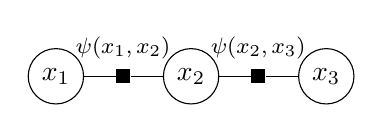
\begin{tikzpicture}
\node[latent] (x1) {$x_1$};
\node[latent, right=of x1] (x2) {$x_2$};
\node[latent, right=of x2] (x3) {$x_3$};
\factor[right=of x1] {f1} {$\psi(x_1,x_2)$} {} {};
\factor[right=of x2] {f2} {$\psi(x_2,x_3)$} {} {};
\factoredge {x1,x2} {f1} {};
\factoredge {x2,x3} {f2} {};
\end{tikzpicture}
\caption{
\label{fig:linear-chain}
}
\end{figure}
\end{comment}
As before, we approximate
$\psi_t(x_{t-1}, x_t) = \exp(\bx_{t-1}^T \bx_t) \approx \phi(\bx_{t-1})^T\phi(\bx_t)$,
with the random projection $\phi(\cdot): \R^n \to \R^d$ chosen appropriately.
To start, consider computing the partition function of a simple example with $T=3$:
\begin{equation}
\begin{aligned}
Z
&= \sum_{x_1}\sum_{x_2} \psi_1(x_1, x_2) \sum_{x_3} \psi_2(x_2, x_3) \\
&\approx \sum_{x_1}\sum_{x_2} \phi(\bx_1)^T\phi(\bx_2) \sum_{x_3} \phi(\bx_2)^T\phi(\bx_3)\\
&= \left(\sum_{x_1} \phi(\bx_1)^T\right) \left(\sum_{\bx_2} \phi(\bx_2)\phi(\bx_2)^T\right)
    \left(\sum_{x_3}\phi(\bx_3)\right).
\end{aligned}
\end{equation}
We can precompute the sum of outer products $\sum_{\bx_2}\phi(\bx_2)\phi(\bx^T)$ independently,
resulting in time complexity $O(Td^2 + T|\mcX|d^2)$ in serial,
and $O(Td^2 + |\mcX|d^2)$ if the sums of outer products can be computed in parallel.
We can also apply a divide-and-conquer approach to further
reduce time to $O(c_{\textrm{mm}}(\log T + \log |\mcX|))$ on a parallel machine,
where $c_{\textrm{mm}}(d)$ is the cost of a matrix multiplication which is polynomial in $d$.
Compared to the original time complexity of $O(T|\mcX|^2)$,
this is particularly beneficial if $d \ll |\mcX|$.

\paragraph{Matrix version}
Probably much clearer here too.
todo

\subsection{Approximation error}
todo

\section{Tree MRFs}
We proceed from first order linear-chain MRFs, where nodes only have 2 neighbours,
to the next simplest model: trees.
With tree MRFs, nodes may have more than 2 neighbours depending on the arity of the tree,
but the dependencies are still simple and exact inference is tractable.

In linear-chain MRFs all elimination orders are equivalent, as the elimination 
of a variable cannot result in the addition of any fill-in edges.
Indeed, this is the reason why divide-and-conquer strategies are possible
in the first place.
As this is not the case for tree MRFs (consider removing a node in the middle of a tree),
it may not be possible to apply the distributive property in order to
improve the time complexity of variable elimination.
However, it may be still be possible to obtain speedups through parallelization. 

\subsection{RFF allows reording of tensor contraction}
Consider a star MRF with the following joint distribution:
\begin{equation}
p(x) \propto \psi(x_1, x_2) \psi(x_2, x_3) \psi(x_2, x_4),
\end{equation}
shown in Figure~\ref{fig:star-mrf}.
\begin{figure}[htb!]
\centering
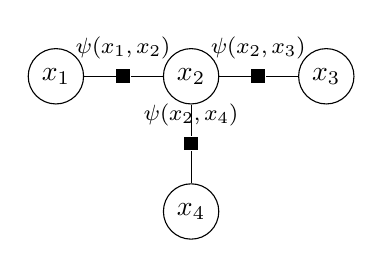
\begin{tikzpicture}
\node[latent] (x1) {$x_1$};
\node[latent, right=of x1] (x2) {$x_2$};
\node[latent, right=of x2] (x3) {$x_3$};
\node[latent, below=of x2] (x4) {$x_4$};
\factor[right=of x1] {f1} {$\psi(x_1,x_2)$} {} {};
\factor[right=of x2] {f2} {$\psi(x_2,x_3)$} {} {};
\factor[below=of x2] {f3} {$\psi(x_2,x_4)$} {} {};
\factoredge {x1,x2} {f1} {};
\factoredge {x2,x3} {f2} {};
\factoredge {x2,x4} {f3} {};
\end{tikzpicture}
\caption{
\label{fig:star-mrf}
}
\end{figure}
Elimination takes time $O(V|\mcX|^2)$, where $V$ is the number of nodes.
The time complexity can be lowered on a parallel device to $O(|\mcX|^2)$
using tensor variable elimination \citep{obermeyer2019tve}.

Applying the RFF approximation, elimination is then given by
\begin{equation}
\begin{aligned}
Z &= \sum_\bz \psi(x_1, x_2) \psi(x_2, x_3) \psi(x_2, x_4) \\
&\approx \sum_{x_1} \sum_{x_2} \phi(x_1)^T\phi(x_2)
    \sum_{x_3} \phi(x_2)^T\phi(x_3) \sum_{x_4} \phi(x_2)^T\phi(x_4)\\
&= \sum_{x_1} \phi(x_1)^T \sum_{x_2} \phi(x_2)
    \left(\phi(x_2)^T \sum_{x_3} \phi(x_3)\right)
    \left(\phi(x_2)^T\sum_{x_4} \phi(x_4)\right).
\end{aligned}
\end{equation}
We can un-distribute $\phi(x_2)^T$ from the last two terms with a tensor product:
\todo{definitely commutative property is being used here, which is clear in the einsum version}
\begin{equation}
Z \approx \left(\sum_{x_1} \phi(x_1)^T \right)
\left(\sum_{x_2} \phi(x_2) \otimes\phi(x_2) \otimes \phi(x_2)  \right)
\left(\sum_{x_3} \phi(x_3)\right) 
\left(\sum_{x_4} \phi(x_4)\right),
\end{equation}
where this approximation can be computed in time $O(|\mcX|d^3)$.

Generalizing to $n$-arity trees, we can go from the original runtime of $O(V|\mcX|^2)$
for variable elimination to $O(Vd^2 + |\mcX|d^n)$ by applying the
RFF approximation and reordering contraction.

\subsection{Approximation error}

\paragraph{Tensor version, einsum version}
\todo{asdf}

\section{Application to Globally Normalized HMMs}
todo

\section{Application to PCFGs}
todo

\bibliographystyle{plainnat}
\bibliography{bib}

\end{document}
